\chapter{Contexte de projet}
\chaptertoc
\vspace{-1.5em}
\section{Introduction}

Ce chapitre présente le cadre général du projet. Il débute par une brève description de l’entreprise d’accueil, \textbf{NTT DATA}. Ensuite, il expose la problématique liée à l’analyse des risques dans les projets pilotés par Jira, ainsi que les objectifs visés. Enfin, il introduit la méthodologie et la planification adoptées.

\section{Organisme d’accueil}

Cette section présente en détail l’organisme d’accueil du projet, en abordant successivement
son historique, ses domaines d’expertise, son organisation interne.

\subsection{Présentation de l’organisme d’accueil}

\textbf{NTT DATA} est une multinationale japonaise spécialisée dans les services informatiques, le conseil technologique et l’intégration de systèmes. Filiale du géant des télécommunications \textbf{Nippon Telegraph and Telephone (NTT)}, l’entreprise opère à l’échelle mondiale pour accompagner la transformation numérique des organisations.

\begin{figure}[!h]
	\centering
	
\includegraphics[width=0.25\linewidth]{assets/Nttdata_log.png}
	\caption{Logo officiel de NTT DATA}
	\label{fig:logo_ntt}
\end{figure}

Au Maroc, NTT DATA accompagne ses clients à travers une gamme complète de services informatiques, articulée autour de quatre axes clés :
\begin{itemize}
	\renewcommand{\labelitemi}{—}
	 \item Conseil en transformation digitale et accompagnement stratégique des projets IT.
    \item  Développement et intégration de solutions logicielles sur mesure (applications d’entreprise, API, microservices).
    \item  Intelligence artificielle et analyse avancée des données (agents conversationnels, LLM, détection de risques, modèles prédictifs).
    \item  Cloud, infrastructure et services managés (conteneurisation Docker, orchestration Kubernetes, CI/CD avec Jenkins).
    \item  Externalisation des processus métier (BPO) et services de recrutement spécialisé.
    \item  Veille économique, analyse et gestion de la performance (tableaux de bord KPI, simulations Monte Carlo).
    \item  Modernisation des systèmes existants et migration vers des architectures cloud hybrides.\end{itemize}

\subsection{Fiche signalétique de l’entreprise}
Ce tableau présente les informations permettant d’identifier l’entreprise NTT DATA.

Le stage s’est déroulé au sein de la filiale marocaine de NTT DATA, située à Casablanca, qui opère sur l’ensemble des métiers de conseil, développement et infrastructure.

\begin{table}[H]
	\centering
	\renewcommand{\arraystretch}{0.9}
	\caption{Fiche signalétique de NTT DATA Maroc (coordonnées et informations clés)}
	\begin{tabular}{|l|l|}
		\hline
		\textbf{Information} & \textbf{Détails} \\
		\hline
		Nom & NTT DATA Maroc \\
		\hline
		Date de création & 2016 \\
		\hline
		Adresse & 5 Boulevard Abdellatif Benkadour, 7ème étage, Casablanca, Maroc \\
		\hline
		Téléphone & +212 5 31 06 29 90 \\
		\hline
		Forme juridique & Société à responsabilité limitée (SARL) \\
		\hline
		Directeur général & Frédéric Sabbah \\
		\hline
		Site Web & \href{https://www.nttdata.com}{www.nttdata.com} \\
		\hline
		Activité & Conseil en systèmes, logiciels informatiques et services numériques \\
		\hline
	\end{tabular}
	\label{tab:fiche_ntt}
\end{table}


\subsubsection{Domaines d’expertise et secteurs d’activité}

La figure suivante \ref{fig:domaines_ntt} présente les principaux domaines d’expertise de NTT DATA Casablanca.

\begin{figure}[H]
	\centering
	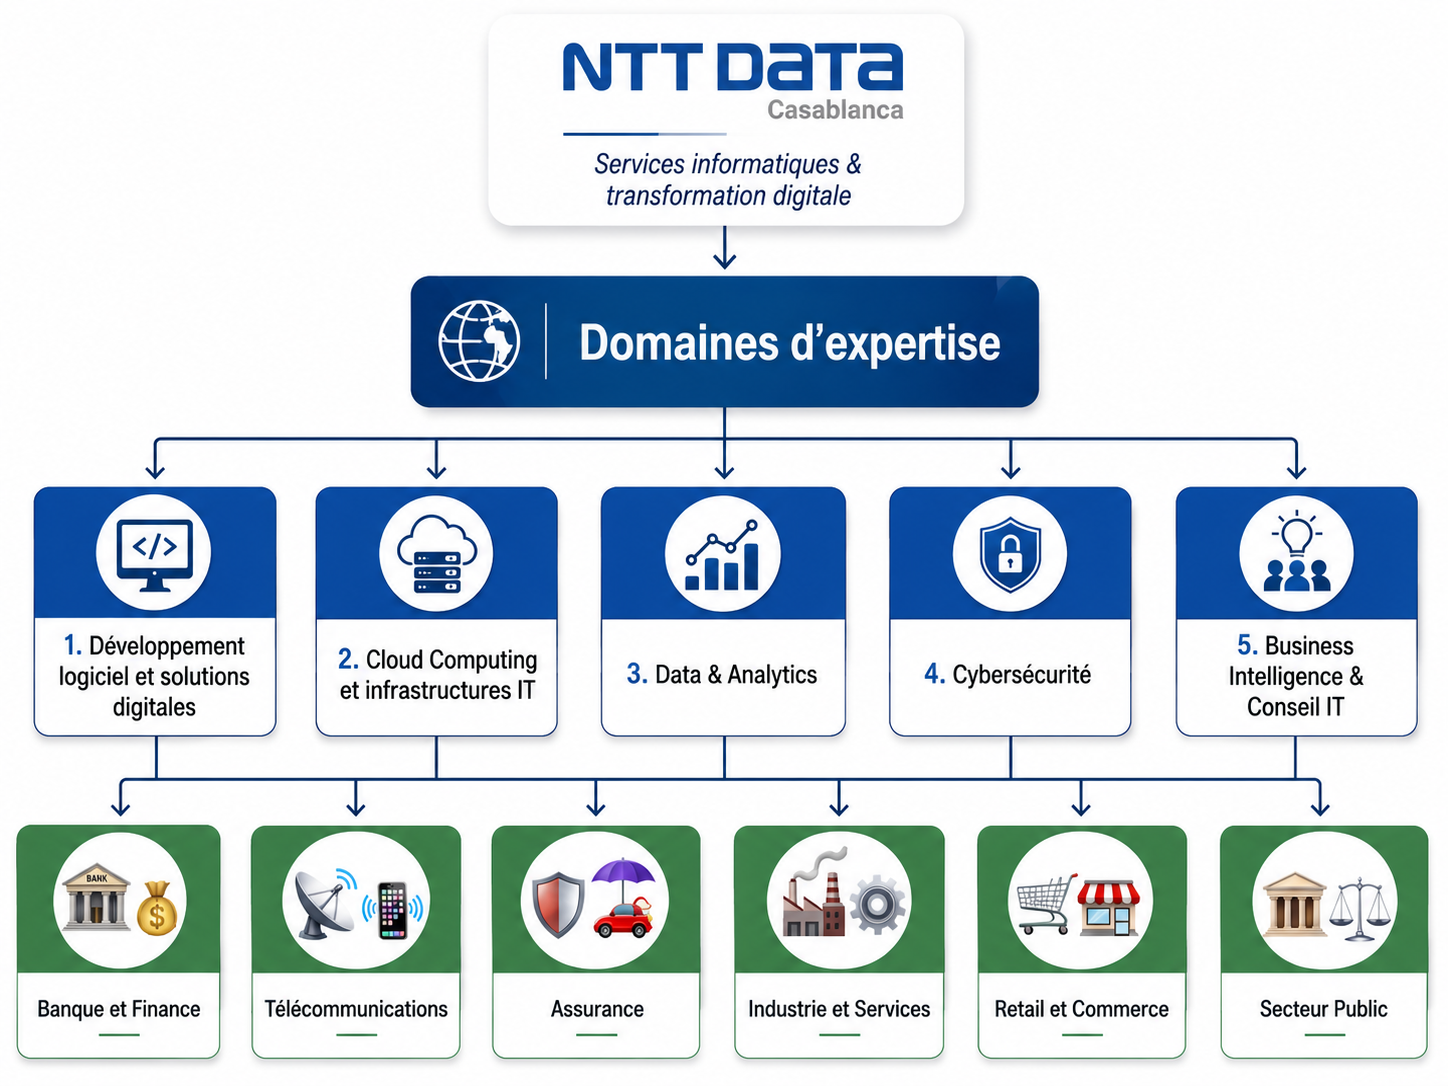
\includegraphics[width=0.8\linewidth]{assets/org.png}
	\caption{Domaines d’expertise et secteurs d’intervention de NTT DATA Casablanca}
	\label{fig:domaines_ntt}
\end{figure}

Comme l’illustre la figure \ref{fig:domaines_ntt}, NTT DATA Maroc structure ses domaines d’expertise autour de cinq pôles principaux :

\begin{enumerate}
    \item \textbf{Développement logiciel et solutions digitales} : conception et réalisation d’applications sur mesure, intégration de systèmes, accompagnement dans la transformation numérique.
    \item \textbf{Cloud Computing et infrastructures IT} : déploiement et gestion d’infrastructures cloud hybrides, migration d’applications, optimisation des ressources.
    \item \textbf{Data \& Analytics} : collecte, traitement et analyse de données massives, mise en place de data lakes, exploitation décisionnelle.
    \item \textbf{Cybersecurity} : audits de sécurité, protection des systèmes d’information, conformité aux normes et régulations.
    \item \textbf{Business Intelligence \& Conseil IT} : tableaux de bord décisionnels, indicateurs de performance, accompagnement stratégique des projets.
\end{enumerate}

L’entreprise intervient principalement dans les secteurs suivants : banque et finance, télécommunications, assurance, industrie et services, retail et commerce, ainsi que le secteur public.

\subsubsection{Présence internationale}
La figure \ref{fig:map_ntt} illustre la présence géographique de NTT DATA à travers le monde.

\begin{figure}[H]
	\centering
	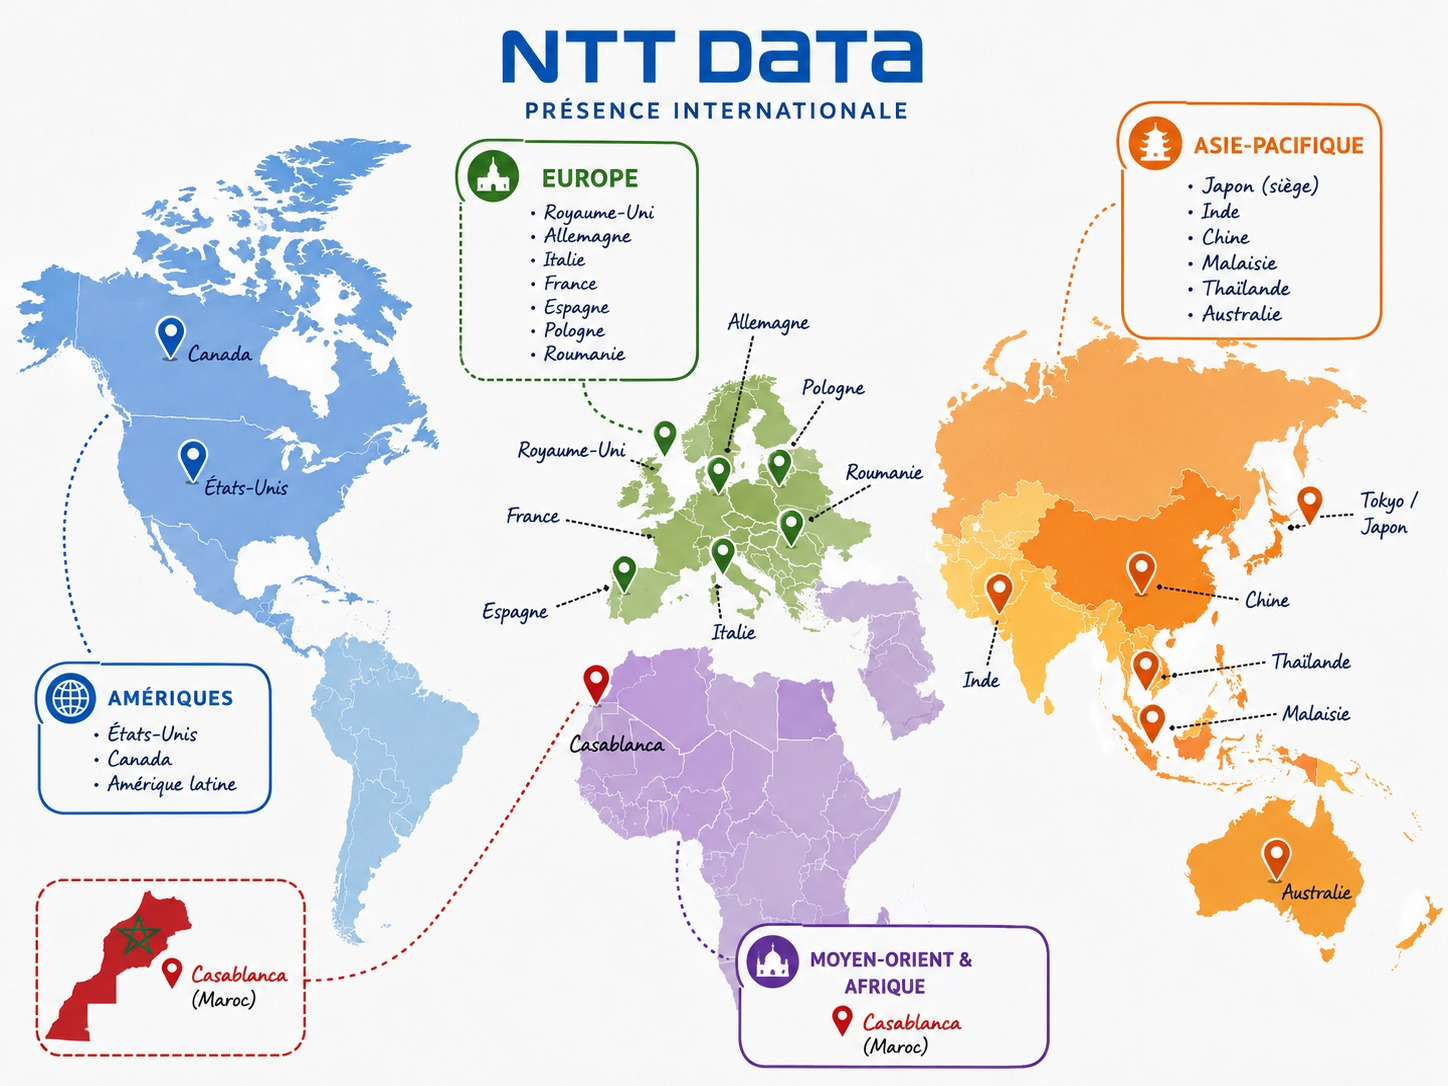
\includegraphics[width=0.8\linewidth]{assets/presence_international.jpeg}
	\caption{Présence géographique de NTT DATA dans le monde}
	\label{fig:map_ntt}
\end{figure}

NTT DATA dispose d’une présence stratégique sur plusieurs continents, avec des bureaux clés notamment :
\begin{itemize}
	\renewcommand{\labelitemi}{—}
	\item \textbf{Tokyo (siège mondial)} : Plus de 150 000 collaborateurs dans le monde
	\item \textbf{Casablanca, Tétouan} : Sièges social pour l’Afrique, moteur de la transformation digitale au Maroc
	\item \textbf{Paris} : Centre européen majeur
	\item \textbf{Washington} : Hub stratégique pour l’Amérique du Nord
	\item \textbf{Dubaï} : Base pour les opérations au Moyen‑Orient
\end{itemize}

\subsection{Structure organisationnelle de l’entreprise}

La Figure \ref{fig:secteurs-nttdata} illustre la structure organisationnelle de la filiale marocaine de NTT DATA. Bien que l'entreprise fasse partie d'un groupe mondial, elle dispose d'une organisation locale agile pour répondre aux enjeux du marché marocain et à ses objectifs de création de plusieurs emplois d'ici 2026.

\begin{figure}[H]
    \centering
    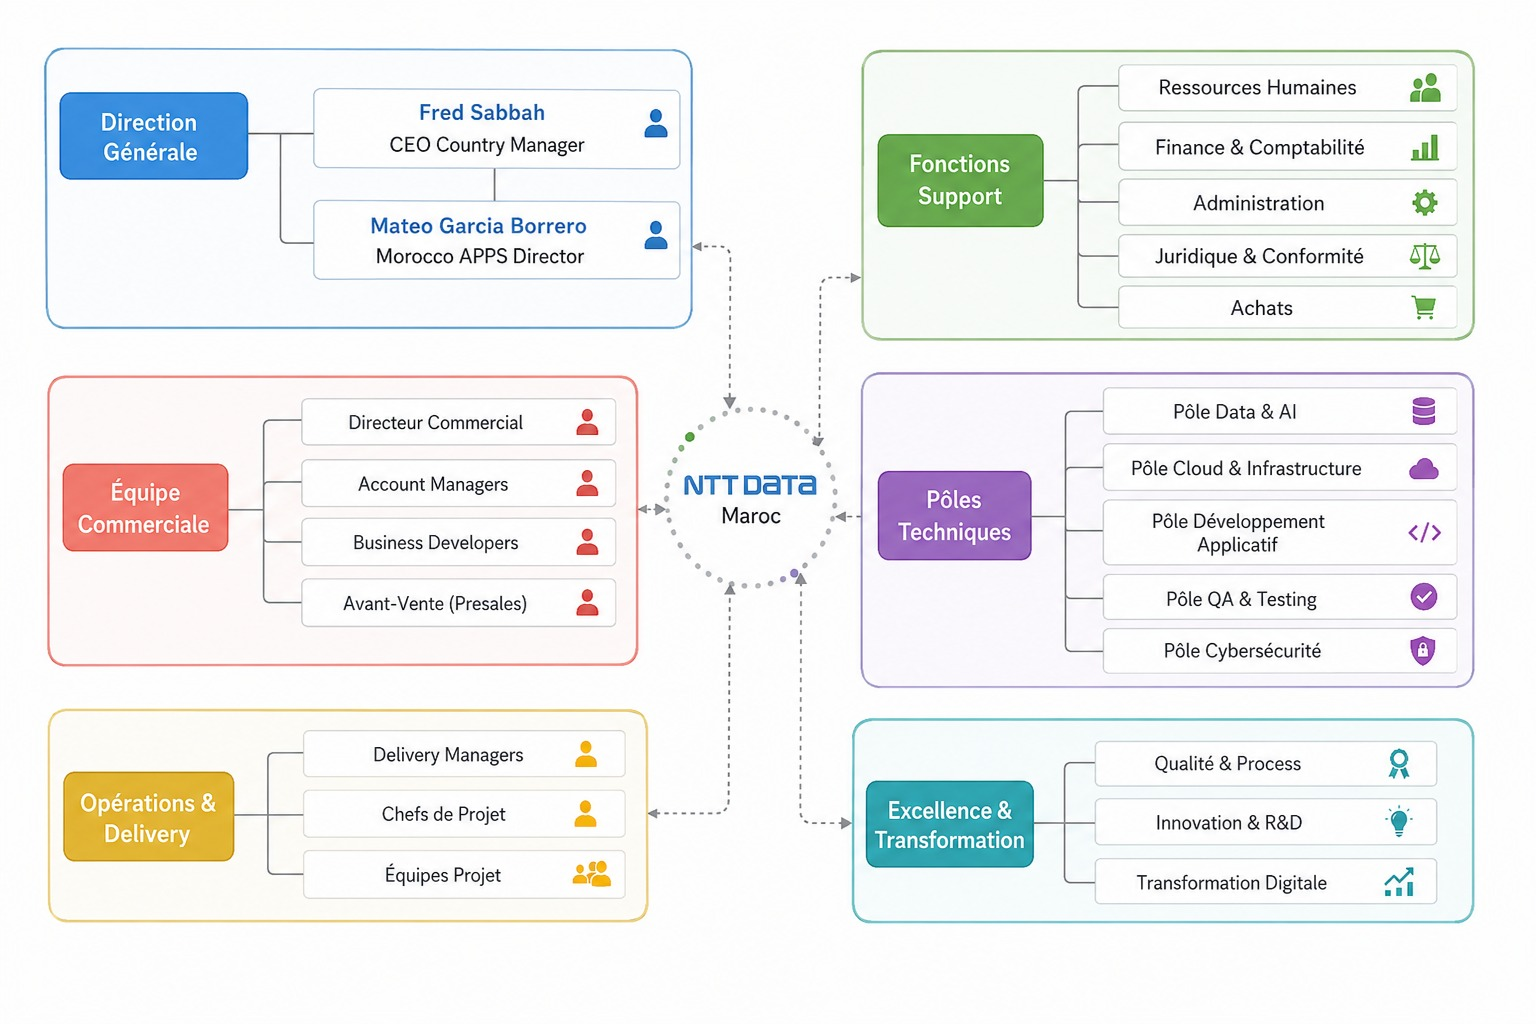
\includegraphics[width=1\linewidth]{assets/logos/secteurs_de_travail.jpeg}
    \caption{Organigramme fonctionnel des principaux pôles de NTT DATA Maroc}
    \label{fig:secteurs-nttdata}
\end{figure}

L'organigramme de NTT DATA Maroc s'articule autour des entités et pôles suivants :

\begin{enumerate}
    \item \textbf{Direction Générale}: Basée à Casablanca, elle est dirigée par le Country Manager, Frédéric Sabbah. Cette équipe définit la vision stratégique et pilote la croissance de l'entreprise au Maroc, en étroite collaboration avec la direction pour la région Moyen-Orient et Afrique.

    \item \textbf{Pôles Techniques et d'Expertise}: Ils constituent le cœur opérationnel de l'entreprise et sont structurés pour délivrer des solutions complètes à ses clients. On y retrouve notamment:
        \begin{itemize}
		\renewcommand{\labelitemi}{—}
            \item Un pôle \textbf{Cloud, Infrastructure et Sécurité}.
            \item Un pôle \textbf{Data \& Intelligence Artificielle (IA)}.
            \item Un pôle dédié aux \textbf{Applications d'entreprise}, avec une expertise particulière sur les solutions SAP.
            \item Un pôle \textbf{Business Process Services (BPS)} pour l'externalisation de processus métier.
        \end{itemize}

    \item \textbf{Équipe Commerciale (Sales) et Marketing}: Chargée du développement du portefeuille clients, de la prospection commerciale et de la gestion des offres de services sur le marché marocain.

    \item \textbf{Équipe des Opérations et du Recrutement}: Essentielle à la stratégie de croissance de l'entreprise, cette équipe gère la livraison des services (notamment pour le pôle BPS) et assure l'acquisition des talents pour atteindre l'objectif ambitieux de création d'emplois.

    \item \textbf{Équipe Administrative et des Ressources Humaines (RH)}: Sous la supervision de la direction, cette équipe gère l'ensemble des aspects financiers, comptables, juridiques et administratifs, ainsi que la gestion du personnel.
\end{enumerate}


\subsection{Contexte interne : utilisation de Jira Data Center}
La gestion de projets logiciels chez NTT DATA génère des volumes croissants de données opérationnelles, principalement via l’outil Jira. Chaque projet peut comporter des centaines, voire des milliers de tickets (tâches, bugs, évolutions), dont l’analyse manuelle pour la détection des risques, des goulots d’étranglement et des retards est devenue trop lente, peu fiable et inadaptée aux exigences de réactivité des équipes. Les chefs de projet et les équipes techniques consacrent un temps considérable à la supervision détaillée de chaque ticket, sans pouvoir bénéficier d’une vision synthétique et prédictive en temps réel.

Face à ce constat, une initiative de modernisation du pilotage de projet a été lancée. L’objectif est de concevoir une plateforme complète, articulée autour d’un \textbf{agent IA conversationnel} comme cœur intelligent, capable d’interagir avec les données Jira de manière autonome et continue. Cette plateforme intègre plusieurs composantes clés :

\begin{itemize}
	\renewcommand{\labelitemi}{—}
    \item Un moteur d’analyse IA qui extrait, normalise et interprète les données Jira pour détecter automatiquement les risques (retards, dépendances critiques, sous-charge ou surcharge d’affectation) et proposer des actions correctives.
    \item Un tableau de bord de monitoring qui offre une vue d’ensemble synthétique, permettant aux responsables de suivre l’état de santé des projets sans avoir à examiner chaque ticket manuellement.
    \item Des simulations Monte Carlo pour prédire la date de fin probable des projets, en prenant en compte l’incertitude des durées et des aléas de développement.
    \item Un explorateur Jira qui structure et visualise les données issues de Jira sous une forme claire et ergonomique.
    \item Un système de contrôle d’accès (RBAC) garantissant que chaque utilisateur (chef de projet, développeur, manager) ne voit que les informations correspondant à son périmètre.
	\item Un système d’alertes automatiques couplé à Microsoft Teams, permettant de notifier instantanément le top management en cas de détection de risque critique.
	\item Une industrialisation complète via un pipeline Jenkins, assurant l’intégration continue, les tests et le déploiement automatisé de la plateforme sur les serveurs de NTT DATA.
	\item Une architecture multi-agents spécialisée, incluant des agents dédiés à l’analyse fine des performances individuelles et collectives (Team Scoreboard et Worker Insights), afin d’optimiser la répartition de la charge de travail.
	\item Une stack d’observabilité technique (Prometheus et Grafana) garantissant la supervision en temps réel de la santé de l’application, des performances du système et des métriques liées à l’intelligence artificielle.
	\item Des métriques avancées et indicateurs de performance (KPIs) permettant d’évaluer en profondeur la dynamique de l’équipe et l’efficacité globale des développements.
\end{itemize}

Cette plateforme répond à un besoin urgent d’accélération de l’analyse : là où une équipe humaine mettrait plusieurs heures ou jours à détecter un risque émergent, l’agent IA opère 24h/24 et 7j/7, fournissant des alertes quasi immédiates. Elle permet également de surmonter les goulots d’étranglement liés à la supervision manuelle détaillée, en libérant du temps pour les tâches à forte valeur ajoutée. Enfin, la capacité prédictive (Monte Carlo) offre une aide à la décision proactive, transformant la gestion de projet réactive en une gestion anticipative et stratégique.

Ainsi, le projet consiste à développer et intégrer l’ensemble de ces briques pour fournir à NTT DATA un outil innovant, permanent et fiable de pilotage de projet par l’IA.

\section{Présentation du projet}
Nous allons à présent détailler le projet sur lequel nous avons travaillé, en commençant par
son contexte, ses enjeux et les objectifs visés.
\subsection{Contexte du projet}

La gestion de projets logiciels chez NTT DATA est en pleine mutation, confrontée à des besoins croissants en matière de réactivité, de fiabilité et d’anticipation des risques. Chaque projet génère des centaines, voire des milliers de tickets Jira (tâches, bugs, évolutions), dont l’analyse manuelle devient trop lente, fastidieuse et inadaptée aux exigences opérationnelles. Dans ce contexte, une initiative de modernisation du pilotage de projet a été lancée pour optimiser la détection des risques et des goulots d’étranglement, en particulier pour les équipes de NTT DATA Maroc.

Cette plateforme innovante se fonde sur le développement d’un \textbf{agent IA conversationnel} capable d’extraire, de normaliser et d’analyser en continu les données issues de Jira. L’objectif global est de fournir aux chefs de projet et aux équipes techniques une vision synthétique et prédictive, avec des alertes automatiques sur les retards, les dépendances critiques et les anomalies d’affectation, ainsi que des recommandations d’actions correctives.

Cette modernisation vise également à répondre à des besoins urgents d’accélération de l’analyse : là où une équipe humaine mettrait plusieurs heures ou jours à détecter un risque émergent, l’agent IA opère 24h/24 et 7j/7, délivrant des informations quasi immédiates. Elle permet de dépasser les limites de la supervision manuelle détaillée, trop lourde à l’échelle de nombreux tickets, et de libérer du temps pour les tâches à forte valeur ajoutée. En raison d’un souci d’implémentation progressive, le projet a été décliné en différentes briques fonctionnelles : tableau de bord de monitoring, simulation Monte Carlo pour la prédiction des dates de fin de projet, explorateur Jira structuré, et système de contrôle d’accès par rôles (RBAC). La première étape concerne notamment l’intégration de l’agent IA conversationnel comme cœur intelligent de la plateforme, pour une détection proactive des risques et des actions recommandées.

\subsection{Problématique du projet}

La gestion des projets logiciels chez NTT DATA, à travers l’outil Jira, constitue un défi opérationnel majeur, notamment lorsque les volumes de données deviennent massifs et que les équipes doivent superviser des centaines de tickets simultanément.

Actuellement, les pratiques d’analyse et de pilotage se heurtent à :
\begin{itemize}
    \renewcommand{\labelitemi}{—}
    \item un volume de données massif (tickets, commentaires, historiques) rendant l’exploitation manuelle fastidieuse.
    \item une hétérogénéité des champs Jira selon les projets, empêchant toute normalisation automatique des informations.
    \item une absence totale de détection automatique des anomalies (tickets bloqués, délais dépassés, dépendances critiques).
    \item une réactivité limitée des équipes de pilotage, contraintes à une supervision séquentielle et chronophage.
    \item une absence de notification instantanée des risques vers le top management, les décisions correctives étant souvent prises avec un retard préjudiciable.
    \item un déploiement manuel des outils de pilotage, sans intégration ni livraison continues, ce qui freine l’industrialisation des solutions.
\end{itemize}

Cela conduit à des risques non identifiés à temps, des retards qui se propagent en cascade, une sous-utilisation des capacités prédictives, une réactivité managériale limitée et une difficulté à maintenir les outils en condition opérationnelle. L’absence d’un mécanisme d’intelligence artificielle capable d’extraire, normaliser et analyser en continu les données Jira, couplé à un pipeline de déploiement automatisé, limite fortement la capacité des équipes à anticiper les problèmes et à proposer des actions correctives rapidement.

La problématique est donc de concevoir une plateforme intelligente, articulée autour d’un agent IA conversationnel, capable d’analyser en temps réel les données Jira, de détecter automatiquement les risques et les goulots d’étranglement, de générer des recommandations actionnables, de notifier instantanément le management (Microsoft Teams) et de s’intégrer dans une chaîne d’industrialisation (Docker, Jenkins). La solution doit également offrir une vision prédictive (Monte Carlo) et un tableau de bord de monitoring adapté aux besoins des chefs de projet et des équipes techniques.


\subsection{Objectifs généraux du projet}

Ce projet vise à moderniser le pilotage des projets logiciels chez NTT DATA à travers la mise en place d’une plateforme full‑stack intelligente, articulée autour d’un agent IA conversationnel, d’un tableau de bord de monitoring, de simulations prédictives, d’une stack d’observabilité et d’un système de contrôle d’accès sécurisé. L’objectif principal est de renforcer la performance et la réactivité des équipes de gestion de projet en leur fournissant des outils d’analyse automatique des risques, de détection des goulots d’étranglement, de prédiction et d’aide à la décision.

La démarche s’articule autour de plusieurs axes stratégiques :

\begin{itemize}
    \renewcommand{\labelitemi}{—}
    \item Développer un agent IA (LangGraph + Mistral) pour l’extraction, la normalisation et l’analyse en continu des données Jira, avec génération automatique de risques et de recommandations.
    \item Concevoir un tableau de bord de métriques et de visualisations (React) offrant aux chefs de projet une vue synthétique et en temps réel de la santé des projets.
    \item Mettre en place une authentification sécurisée par rôles (RBAC, JWT, PostgreSQL) pour garantir la confidentialité et la granularité des accès selon les profils utilisateurs.
    \item Intégrer un cache Redis pour optimiser les performances d’accès aux données fréquemment sollicitées.
    \item Industrialiser la solution via Docker (conteneurisation) et Jenkins (intégration et déploiement continus).
    \item Déployer une stack de supervision (Prometheus, Grafana, Alertmanager) pour collecter les métriques système et applicatives, visualiser la santé des projets en temps réel et déclencher des alertes.
    \item Mettre en place un système de notification automatique vers Microsoft Teams afin d’alerter instantanément le top management en cas de risque critique.
    \item Développer un tableau de bord des performances individuelles (Team Scoreboard) permettant d’analyser la charge, la vélocité et la productivité de chaque membre de l’équipe.
\end{itemize}

\subsection{Objectifs spécifiques de la plateforme IA}

Dans cette première phase, l’objectif est de développer une solution dédiée à l’analyse automatique des risques projet à partir des tickets Jira.

La solution devra :

\begin{itemize}
    \renewcommand{\labelitemi}{—}
    \item Extraire et normaliser les tickets Jira via l’API REST, en gérant l’hétérogénéité des champs entre les projets.
    \item Calculer des signaux de santé projet (WIP ratio, stale ratio, overdue rate, coefficient de Gini) à partir des données historiques et en temps réel.
    \item Implémenter un moteur de règles combiné à un LLM (Mistral hébergé à Tétouan, accessible via API) pour générer des risques, des actions correctives et des recommandations contextuelles.
    \item Fournir une interface React avec visualisations de métriques, un explorateur Jira structuré et un tableau de bord des performances individuelles.
    \item Assurer la sécurité des échanges (JWT) et la gestion fine des rôles utilisateurs.
    \item Conteneuriser l’application avec Docker et orchestrer le déploiement via Jenkins.
    \item Implémenter des simulations de Monte Carlo pour prédire la date de fin des projets en fonction de la vélocité historique et du backlog restant (percentiles p50 à p95).
    \item Superviser l’état de santé de l’application via Prometheus et Grafana, avec des règles d’alerte personnalisées (ex. \texttt{CriticalWipRatio}, \texttt{ProjectAtRisk}).
\end{itemize}

L’approche proposée repose sur l’utilisation d’algorithmes d’intelligence artificielle et d’un agent conversationnel capable d’opérer 24h/24 et 7j/7, couplé à une stack d’observabilité moderne, permettant non seulement de réduire les délais de détection des anomalies, mais aussi d’anticiper les retards, d’alerter proactivement le management et de maximiser la réactivité des équipes de pilotage.
Ce travail constitue une première brique essentielle, posant les bases techniques et méthodologiques sur lesquelles s’appuieront les prochaines phases du projet, visant à étendre l’analyse prédictive (simulations Monte Carlo) et l’optimisation à d’autres dimensions de la gestion de projet (budget, ressources humaines, qualité logicielle).

\subsection{Conduite du projet}

Cette section présente la méthodologie et la planification du projet, en décrivant les approches et étapes clés pour sa réussite.

\subsubsection{Méthodologie de travail}

La méthodologie adoptée est Scrum, une approche agile itérative qui facilite le suivi du projet, encourage l’adaptabilité, la collaboration et l’amélioration continue à travers des sprints courts.

\begin{figure}[H]
	\centering
	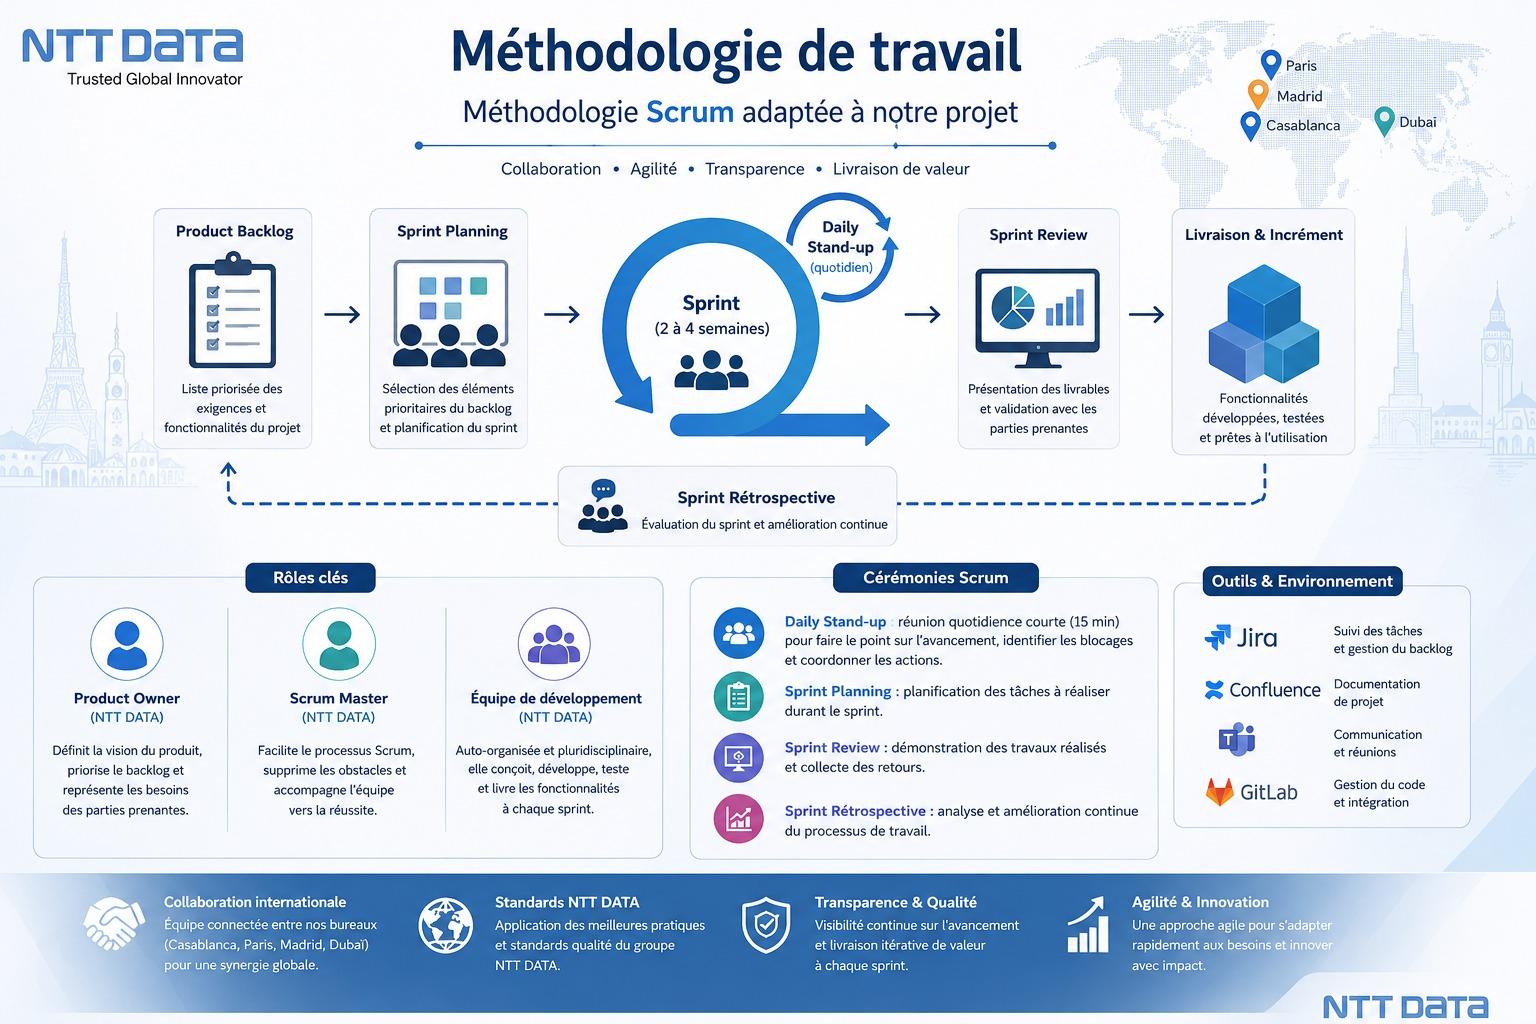
\includegraphics[width=0.8\linewidth]{assets/methodologie_travail.jpeg}
	\caption{Méthodologie agile Scrum adoptée pour le projet}
	\label{fig:scrum_ntt}
\end{figure}

\paragraph{Les rôles Scrum dans notre projet}

Les trois rôles principaux dans notre projet sont les suivants :

\begin{itemize}
	\renewcommand{\labelitemi}{—}
	\item \textbf{Product Owner} : Le top management de NTT DATA Maroc (direction générale), responsable de la vision stratégique, du backlog prioritaire et de la validation des livrables.
	\item \textbf{Scrum Master} :  Mohammed Amine Elmeknassi, supervise le processus Scrum, organise les réunions quotidiennes, répartisse les tâches et identifient les blocages.
	\item \textbf{Équipe Intelligence Artificielle} : composée de moi-même, Nour Derraz et Image Chaoui, responsable de la conception de l’agent IA, du développement de la plateforme full‑stack, de l’analyse des données Jira et de la documentation technique.
\end{itemize}

\paragraph{Cérémonies Scrum}

Chaque jour, de 9h à 9h45, nous tenons un \textbf{Daily Stand-up} à distance (visioconférence) avec Mohammed Amine Elmeknassi. Cette réunion sert à faire le point sur l’avancement, identifier les blocages et coordonner les actions. La majorité du travail s’effectue à distance, avec une présence physique au bureau de NTT DATA Casablanca une fois par semaine pour les réunions de synthèse.

Chaque semaine, nous produisons une présentation (PPT) listant l’ensemble des réalisations accomplies. Mohammed Amine Elmeknassi transmet ce compte rendu à Anis Khairi, puis ils le remontent au top management de NTT DATA Maroc afin de suivre l’avancement global du projet.

Avant chaque sprint, la \textbf{Sprint Planning Meeting} permet de sélectionner les éléments prioritaires du Product Backlog à développer. La \textbf{Sprint Review} présente les fonctionnalités développées aux parties prenantes, notamment le top management de NTT DATA Maroc et les responsables techniques.

\subsubsection{Planification du projet}

Bien que Scrum repose sur une gestion itérative des priorités, un diagramme de Gantt a été utilisé pour visualiser les grandes étapes du projet (développement de l’agent IA, intégration de l’API Jira, mise en place du tableau de bord, simulation Monte Carlo, RBAC, déploiement Docker/Jenkins), leur enchaînement et leurs dépendances.
\begin{figure}[H]
	\centering
	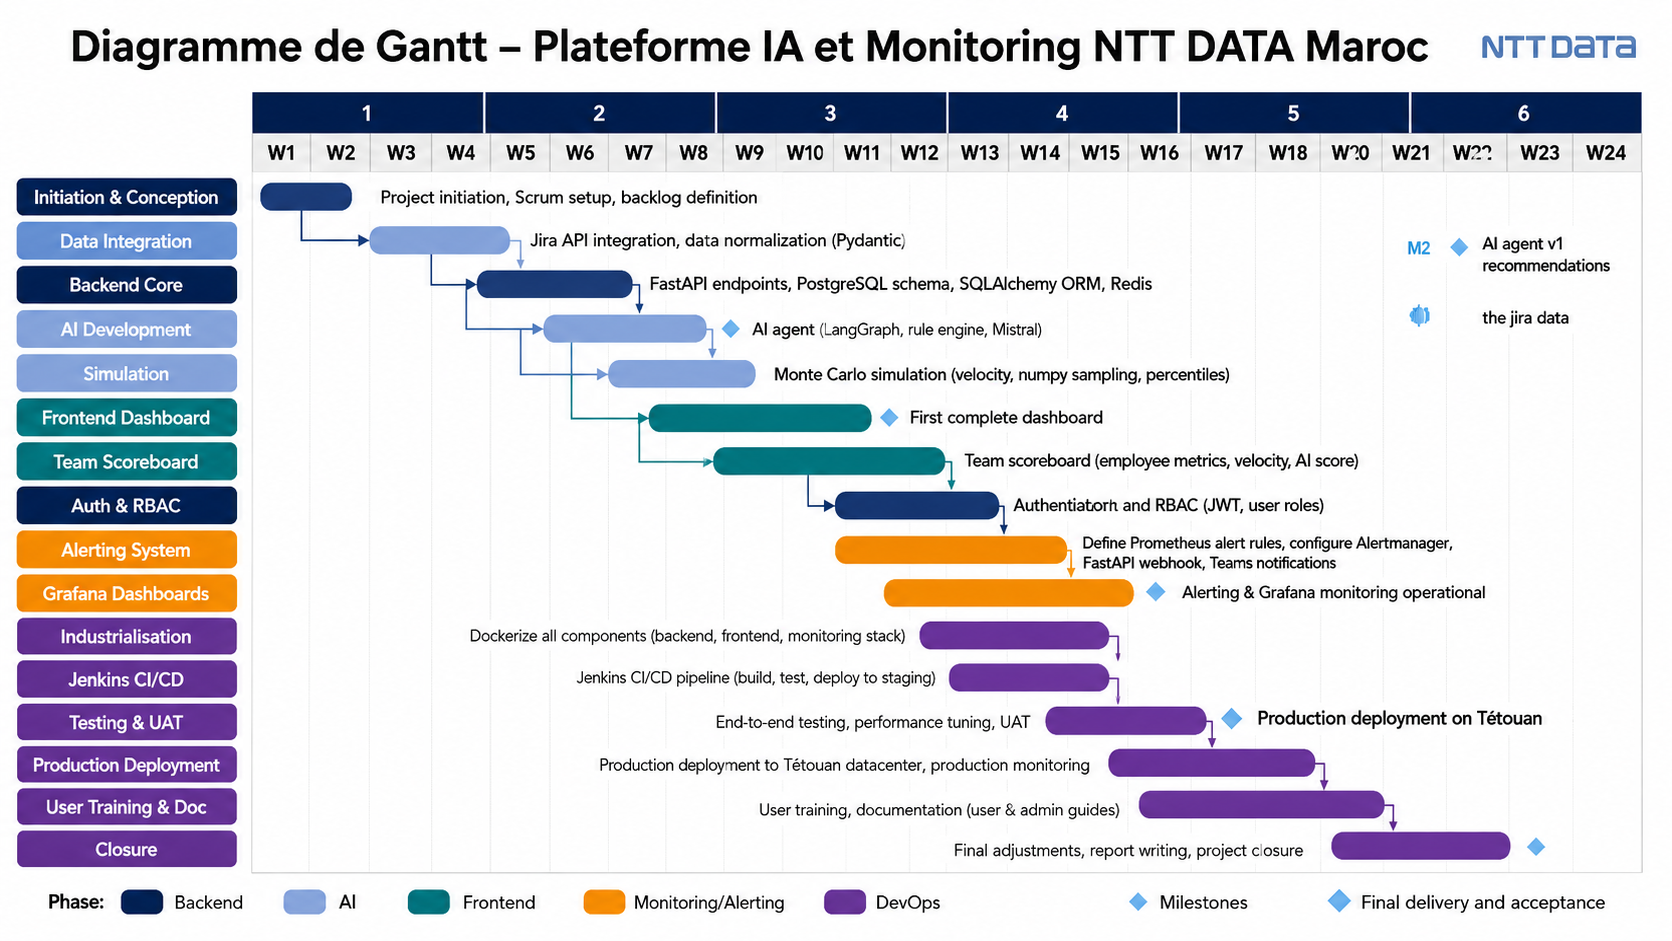
\includegraphics[width=0.8\linewidth]{assets/diagram_gant.png}
	\caption{Diagramme de Gantt illustrant la planification globale du projet}
	\label{fig:gant_ntt}
\end{figure}


\section{Conclusion}

Pour conclure ce premier chapitre, nous avons présenté NTT DATA Maroc en soulignant son contexte historique, son activité et sa structure organisationnelle. Nous avons également exposé la problématique du projet – la lenteur et le manque de fiabilité de l’analyse manuelle des tickets Jira – ainsi que les objectifs généraux et spécifiques de la plateforme à agent IA. Enfin, nous avons abordé la méthodologie Scrum adoptée, les rôles de l’équipe, les cérémonies quotidiennes et hebdomadaires, ainsi que la planification globale. Dans le prochain chapitre, nous aborderons l’analyse des besoins, la conception fonctionnelle ainsi que l’architecture technique du projet.